
\section{Using the Human Player GUI}\label{ch:usingHI} 

When the GUI is open (Figure \ref{fig:humanPlayerGUI}), two main parts can be seen:
\begin{enumerate}
\item The map panel, where the map and the block sequence are being displayed.
\item The message panel, where the remaining bot battery and messages between bots and e-partner are being displayed. Messages can be be sent to other bots and your e-partner.
\end{enumerate}


\begin{figure}[h]
\begin{center}
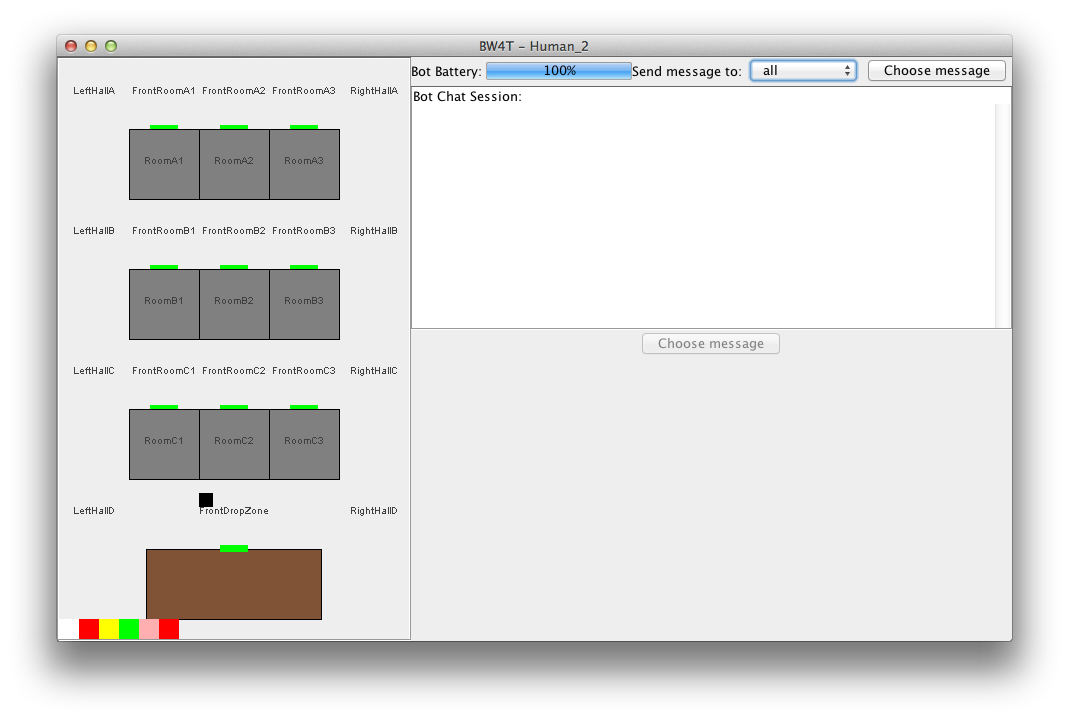
\includegraphics[width = 0.8\textwidth]{HumanPlayerGUI/hpg.png}
\caption{Human Player GUI with map panel (left) and message panel (right).}
\label{fig:humanPlayerGUI}
\end{center}
\end{figure}

\subsection{General use}
To use the human player interface (Figure \ref{fig:humanPlayerGUI}), the user clicks with the left (occasionally the right) mouse button in the GUI. Depending on where the user clicks, different menus appear. The user then picks the appropriate action from the menu to execute that action. Below the possibilities are explained.

On the left side of the interface, the bot can be directed by clicking on the map. Different pop-up menus will appear upon clicking on different entities on the map.

On the right side of the interface, the battery capacity of the bot that can be controlled can be found. Bots can be selected to which messages need to be sent and messages can be sent here. The bot chat session and the e-partner chat session are also displayed.


\subsection{Map Panel}
A picture of the Map Panel is shown in \ref{fig:mapPanel}.

\begin{figure}[h]
\begin{center}
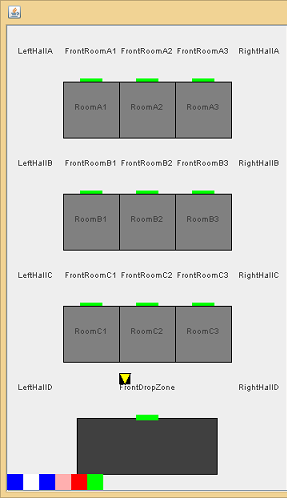
\includegraphics[width= 0.35\textwidth]{HumanPlayerGUI/hpg-left.png}
\end{center}
\caption{Map Panel}
\label{fig:mapPanel}
\end{figure}

Here the following actions can be done:

\begin{itemize}

\item \textbf{Go to: $"place"$}:
To command the controlled bot to go to a room or a certain place in the corridors, click on the room or place where the bot needs to go to. The corridor menu (figure ~\ref{fig:corridorMenu}) will appear next to your mouse pointer with the option $go$ $to$ $here$ or $Go$ $to$ $"room"$.\\

\begin{figure}[h]
\centering
\begin{minipage}{0.48\textwidth}
	\centering
	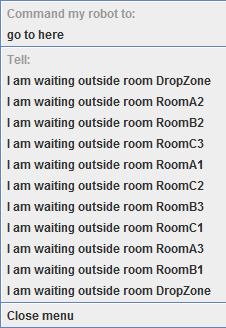
\includegraphics[width=0.5\textwidth]{HumanPlayerGUI/hpg-corridor-menu.png}
	\caption{Corridor menu}
	\label{fig:corridorMenu}
\end{minipage}\hfill
\begin{minipage}{0.48\textwidth}
	\centering
	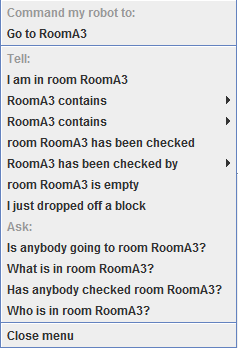
\includegraphics[width=0.5\textwidth]{HumanPlayerGUI/hpg-room-menu.png}
	\caption{Room menu}
	\label{fig:roomMenu}
\end{minipage}
\end{figure}


\item \textbf{Send message: I am waiting outside $"room"$}:
To send a message to a bot or to all bots, click in the corridor. The corridor menu (figure ~\ref{fig:corridorMenu}) will appear next to your mouse pointer with the options $I$ $am$ $waiting$ $outside$ $"room"$. A message will be send to all bots by default. To see how to change the receiver of the messages, go to the Message Panel section.

\item \textbf{Send message: I am in $"room"$}:
To send a message to a bot or to all bots, click in the room. The room menu (figure \ref{fig:roomMenu}) will appear next to your mouse pointer with the option: I am in $"room"$. A message will be send to all bots by default. To see how to change the receiver of the messages, go to the Message Panel section.

\item \textbf{Send message: tell other bot(s) $"information"$}:
To send a message to a bot or to all bots with certain information about a certain room, click on the room. The room menu (Figure \ref{fig:roomMenu}) will appear next to your mouse pointer with the messages you can send. A message will be send to all bots by default. To see how to change the receiver of the messages, go to the Message Panel section.

\item \textbf{Send message: ask other bot(s) $"question"$ about certain room}:
To ask a bot or all bots a question about a certain room, click on the room. The room menu (Figure \ref{fig:roomMenu}) will appear next to your mouse pointer with the possible questions that can we asked. A message will be send to all bots by default. To see how to change the receiver of the messages, go to the Message Panel section.

\item \textbf{Pick up block}:
To pick up a $"block"$, click on the block that needs to be picked up. The block menu (Figure \ref{fig:blockMenu}) will appear next to your mouse pointer. Click on $Go$ $to$ $"color"$ $block$. When the controlled bot is standing on the block, click on the bot. The block menu when standing on block (Figure \ref{fig:blockMenu2}) will appear. Click on $Pick$ $up$ $"color"$ $block$.

\begin{figure}[h]
\centering
\begin{minipage}{0.5\textwidth}
\centering
  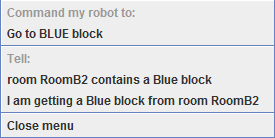
\includegraphics[width=.8\linewidth]{HumanPlayerGUI/hpg-block-menu1.png}  
  \caption{Block menu} \label{fig:blockMenu}
\end{minipage}\hfill
\begin{minipage}{0.5\textwidth}
  \centering
  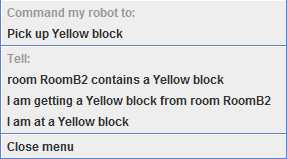
\includegraphics[width=.8\linewidth]{HumanPlayerGUI/hpg-block-menu2.png}
  \caption{Block menu when standing on block} \label{fig:blockMenu2}
\end{minipage}
\end{figure}

\item \textbf{Drop block}:
To drop the block that is currently being held, click on the room in which it needs to be dropped. The room menu when holding block will appear next to your mouse pointer. This menu is almost identical to (Figure \ref{fig:roomMenu} but it has an extra item 'Put down block'). Click on $Put$ $down$ $block$. Do note that the controlled bot should be in the same room as where you want to drop the block.


\item \textbf{Pick up e-partner}:
To pick up an e-partner, click on the e-partner that needs to be picked up. The e-partner menu (Figure \ref{fig:epartnerMenu}) will appear next to your mouse pointer. Click on $Go$ $to$ $e-partner$. When the controlled bot is standing on the e-partner, click on the e-partner again. The e-partner menu when standing on e-partner (Figure \ref{fig:epartnerMenu2}) will appear. Click on $Pick$ $up$ $e-partner$.

\begin{figure}[h]
\begin{minipage}{0.48\textwidth}
  \centering
  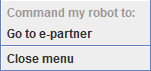
\includegraphics[width=.5\linewidth]{HumanPlayerGUI/hpg-epartner-menu1.png}
  \caption{The e-partner menu}
  \label{fig:epartnerMenu}
\end{minipage}\hfill
\begin{minipage}{0.48\textwidth}
  \centering
  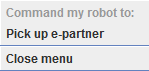
\includegraphics[width=.5\linewidth]{HumanPlayerGUI/hpg-epartner-menu2.png}
  \caption{E-partner menu when standing on e-partner}
  \label{fig:epartnerMenu2}
\end{minipage}
\end{figure}

\item \textbf{Send message to e-partner}:
To send a message to the e-partner that is currently being held, click on the e-partner. The e-partner menu when holding e-partner (Figure  \ref{fig:epartnerMenu3}) will appear next to your mouse pointer. Click on $I$ $am$ $going$ $to$ $"room"$. This option will only appear if the e-partner has GPS enabled.

\begin{figure}
\begin{center}
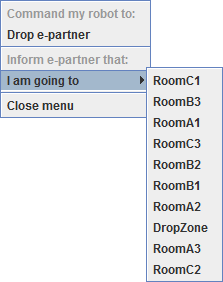
\includegraphics{HumanPlayerGUI/hpg-epartner-menu3.png}
\end{center}
\caption{E-partner menu when holding e-partner}
\label{fig:epartnerMenu3}
\end{figure}

\item \textbf{Drop e-partner}:
To drop the e-partner which is currently being held, click on the e-partner. The e-partner menu when holding e-partner (figure  \ref{fig:epartnerMenu3}) will appear next to your mouse pointer. Click on $Put$ $down$ $e-partner$.

\end{itemize}


\subsection{Sending messages}
By clicking on the drop-down menu, the user can choose to which bot he or she will send a request or question. "all" sends the message to all bots. Next to the drop-down menu, a button is placed with choose message. This button contains the messages that are most likely to be sent. Left clicking this button will create a list from which the user can choose a message. The "Bot Chat Session" menu ives a number of standard answers: yes, no, don't know, ok, etc. It is not possible to use free text because the non-human agents can only process these pre-specified messages. The specification document gives more details on how messages are processed by non-human agents.

\subsection{Click on room or dropzone}
By clicking on a room, the user can order his bot to go to that room, tell everybody something about that room or ask something about that room.
\subsection{Click on blocks}
By clicking on a block (particularly, those below the drop zone), the user can tell everybody something about that block, or ask others for information about that block.
\subsection{Click on hallway}
By clicking on a hallway, the user can point to an exact (X,Y) location to go to. Also it is possible to tell all others roughly where one is in the hallway.


\subsection{The message panel}
A picture of the Message Panel can be found in figure ~\ref{fig:mp1}. The second choose message button will only be enabled when the bot is holding an e-partner. Below this button, the e-partner chat session will appear when the bot holds an e-partner for the first time. Figure ~\ref{fig:mp2} shows the Message Panel when the e-partner has been held and dropped.
\\
\begin{figure}[h]
\begin{center}
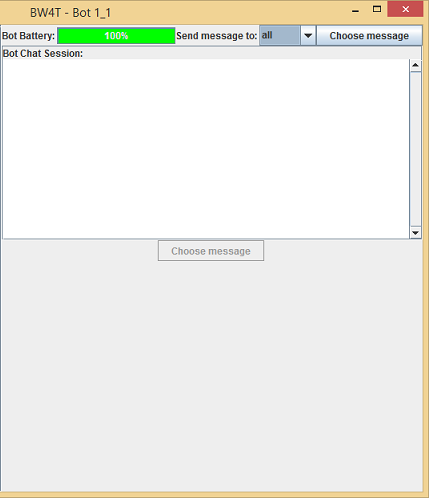
\includegraphics{HumanPlayerGUI/hpg-right.png}
\end{center}
\caption{Message Panel}
\label{fig:mp1}
\end{figure}

\begin{figure}[h]
\begin{center}
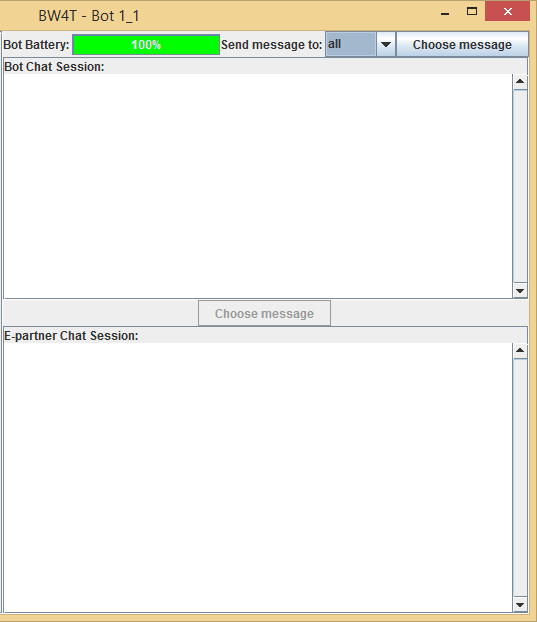
\includegraphics{HumanPlayerGUI/hpg-right-epartner.png}
\end{center}
\caption{Message Panel with e-partner section}
\label{fig:mp2}
\end{figure}

\textbf{Select message receiver}
To select who a message needs to be sent to, click on the dropdown box (Figure ~\ref{fig:receiverDropDown}) at $Send$ $message$ $to:$. The receiver is by default $all$.
When set to $all$, all other bots receive the message. When set to a specific bot, only that bot receives the message.
\\
\begin{figure}[h]
\begin{center}
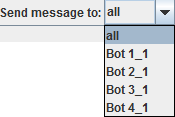
\includegraphics{HumanPlayerGUI/hpg-bot-receiver.png}
\end{center}
\caption{Select receiver dropdown}
\label{fig:receiverDropDown}
\end{figure}

\textbf{Send message to bot(s)}
To send a message, click on the $Choose$ $message$ button. A menu (figure ~\ref{fig:messageBot}) will appear next to your mouse pointer with the possible messages to be sent.
\\
\begin{figure}[h]
\begin{center}
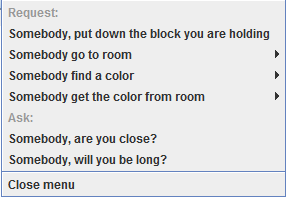
\includegraphics{HumanPlayerGUI/hpg-bot-message.png}
\end{center}
\caption{Choose message button menu}
\label{fig:messageBot}
\end{figure}

\textbf{Answer a question}
To answer questions asked by other bots, click in the bot chat session box. A menu (figure ~\ref{fig:answerBot}) will appear next to your mouse pointer with the possible answers to be sent.
\\
\begin{figure}[h]
\begin{center}
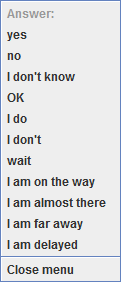
\includegraphics{HumanPlayerGUI/hpg-bot-chat.png}
\end{center}
\caption{Bot answer menu}
\label{fig:answerBot}
\end{figure}

\textbf{Send message to e-partner}
To send a message to the e-partner that is currently being held, click on the choose message button. A menu (figure  ~\ref{fig:epartnerMenu3}) will appear next to your mouse pointer. Click on $I$ $am$ $going$ $to$ $"room"$. This option will only appear if the e-partner has GPS enabled.
\\
\textbf{Drop e-partner}
To drop the e-partner that is currently being held, click on the choose message button. A menu (figure  ~\ref{fig:epartnerMenu3}) will appear next to your mouse pointer. Click on $Drop$ $e-partner$. The choose message button will be disabled after dropping the e-partner.